\chapter{Variables}
\label{c:var}
\index{variables}

%-------------------------------------------------------------------------------
\section{Overview}
\label{s:var.overview}

\tao defines objects called \vn{variables} whose main purpose is to enable optimizations
(\sref{c:opti}). Essentially, a variable acts as as a controller for a lattice parameter. For
example, a variable may control the \vn{k1} quadrupole strength of a particular lattice element.
Another use for variables is that a block of variables can be plotted for visual inspection.
\vn{Variables} can be defined in the \tao initialization files (\sref{s:init.var}).

%-------------------------------------------------------------------------------
\begin{figure}
  \centering
  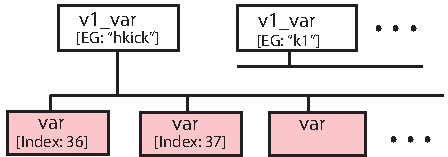
\includegraphics[width=4in]{var-tree.pdf}
  \caption[VAriable tree structure]
{A \vn{v1_var} structure holds an array of variables. Illustrated is a \vn{var_var} structure
holding an array of variables with each variable controlling the \vn{hkick} attribute of a
particular lattice element.}
  \label{f:var.tree}
\end{figure}

%-------------------------------------------------------------------------------

\index{variables!v1_var}
Blocks of variables are associated with what is called a \vn{v1_var} structure as illustrated in
Figure~\ref{f:var.tree}. Each \vn{v1_var} structure defined has a \vn{name} with which to refer to
in \tao commands. For example, if ``\vn{quad_k1}'' is the name of a \vn{v1_var}, then
\vn{quad_k1[5]} references the variable with index 5 in the array associated with the \vn{quad_k1}
\vn{v1_var} structure.

A set of variables within a \vn{v1_var} block can be referred to by using using a comma \vn{,} to
separate their indexes. Additionally, a Colon ``\vn{:}'' can be use to specify a range of
variables. For example
\begin{example}
  quad_k1[3:6,23]
\end{example}
refers to variables 3, 4, 5, 6, and 23. Instead of a number, the associated lattice element name can
be used so if, in the above example, the lattice element named \vn{q01} is associated with
\vn{quad_k1[1]}, etc., then the following is equivalent:
\begin{example}
  quad_k1[q03:q06,q23]
\end{example}
Using lattice names instead of numbers is not valid if the same lattice element is associated with
more than one variable in a \vn{v1_var} array. This can happen, for example, if one variable
controls an element's \vn{x_offset} and another variable controls the same element's \vn{y_offset}.

In referring to variables, a ``\vn{*}'' can be used as a wild card to 
denote ``all''. Thus:
\begin{example}
  *                 ! All the variables
  quad_k1[*]|design ! All design values of quad_k1.
  quad_k1[]|model   ! No values. That is, the empty set.
  quad_k1|model     ! Same as quad_k1[*]|model
\end{example}

%-------------------------------------------------------------------------------
\section{Anatomy of a Variable}
\label{s:var.anatomy}

A given variable may control a single parameter of one element (or \vn{particle_start}) in a
\vn{model} lattice of a single universe or it can be configured to simultaneously control an element
attribute across multiple universes. Any one variable cannot control more than one attribute of one
element. However, a variable may control an overlay or group element which, in turn, can control
numerous elements.

Each individual variable has a number of values associated with it: The list of components that can
be set or refereed to are:
\begin{example}
  ele_name     ! Associated lattice element name.
  attrib_name  ! Name of the attribute to vary.
  ix_attrib    ! Index in ele%value(:) array if appropriate.
  s            ! longitudinal position of ele.

  meas         ! Value of variable at time of a data measurement.
  ref          ! Value at time of the reference data measurement.
  model        ! Value in the model lattice.
  base         ! Value in the base lattice.
  design       ! Value in  the design lattice.
  correction   ! Value determined by a fit to correct the lattice.
  old          ! Scratch value.

  weight       ! Weight used in the merit function.
  delta_merit  ! Diff used to calculate the merit function term.
  merit        ! merit_term = weight * delta^2.
  merit_type   ! "target" or "limit"
  dMerit_dVar  ! Merit derivative.

  high_lim     ! High limit for the model_value.
  low_lim      ! Low limit for the model_value.
  step         ! For fitting/optimization: What is considered a small change.

  key_bound    ! Variable bound to keyboard key?
  ix_key_table ! Has a key binding?

  ix_v1        ! Index of this var in the s%v1_var(i)%v(:) array.
  ix_var       ! Index number of this var in the s%var(:) array.
  ix_dvar      ! Column in the dData_dVar derivative matrix.

  exists       ! Does the variable exist?
  good_var     ! The variable can be varied (set by \tao).
  good_user    ! The variable can be varied (set by the user).
  good_opt     ! For use by extension code.
  good_plot    ! Is variable within the horizontal extent of the plot? 
  useit_opt    ! Variable is to be used for optimizing.
  useit_plot   ! Variable is to be used for plotting.
\end{example}

  \index{variable!measured}\index{variable!reference}
  \index{variable!model}\index{variable!design}\index{variable!base}
  \begin{description}
  \item[attrib_name] \Newline
Name of the attribute to vary. Consult the \bmad manual for appropriate attribute names. If the
attribute is associated with a lattice element, the \vn{show element -all} command will list most
attributes of interest.  It is important to keep in mind that it is not possible to use attributes
that are computed (that is, dependent attributes).
  \item[base] \Newline
The value of the variable as derived from the \vn{base} lattice (\sref{s:universe}).
  \item[delta_merit] \Newline
Difference value used to calculate the contribution of the variable to the merit function (\Eq{m1}).
  \item[design] \Newline
The value of the variable as given in the \vn{design} lattice.
  \item[dMerit_dVar] \Newline
Derivative of the merit function with respect to the variable.
  \item[ele_name] \Newline
Associated lattice element name. For controlling the starting position in a lattice with open
geometry the element name is \vn{particle_start} (which is the name used if the starting position is
set in the lattice file). 
  \item[exists] \Newline
The variable exists. Non-existent variables can serve as place holders in a variable
array.
  \item[good_opt] \Newline
Logical not modified by Tao proper and reserved for use by extension code. See below.
  \item[good_plot] \Newline
Set by Tao. Is variable point within the horizontal extent of the plot? 
  \item[good_var] \Newline
Logical controlled by \tao and used to veto variables that should not be varied during
optimization. For example, variables that do not affect the merit function. See below.
  \item[good_user] \Newline
Logical set by the user using \vn{veto}, \vn{use}, and \vn{restore} commands to indicate
whether the variable should be used when optimizing. See below.
  \item[high_lim] \Newline
High limit for the model value during optimization (\sref{s:del.v}) beyond which
the contribution of the variable to the merit function is nonzero.
  \item[ix_attrib] \Newline
Index assigned by \bmad to the attribute being controlled. Used for diagnosis and not
of general interest.
  \item[ix_dvar] \Newline
Column index of the variable in the dData_dVar derivative matrix constructed by \tao.
Used for diagnostics and not of general interest.
  \item[ix_key_table] \Newline
Index of the variable in the key table (\sref{s:key.bind}).
  \item[ix_v1] \Newline
Index of this variable in the variable array of the associated \vn{v1_var} variable.
For example, a variable named \vn{q1_quad[10]} would have \vn{ix_v1} equal to 10.
  \item[ix_var] \Newline
For ease of computation, \tao establishes an array that holds all the variables.
\vn{ix_var} is the index number for this variable in this array. 
Used for diagnostics and not of general interest.
  \item[key_bound] \Newline
Variable bound to keyboard key (\sref{s:key.bind})?
  \item[measured] \Newline
The value of the variable as obtained at the time of a \vn{data} measurement.
  \item[merit] \Newline
The contribution to the merit function \Eq{m1} from the variable. Use the \vn{show merit}
command to set the variables and data which contribute most to the merit function.
  \item[merit_type] \Newline
"target" or "limit".
  \item[low_lim] \Newline
Lower limit for the model value during optimization (\sref{s:del.v}) beyond which
the contribution of the variable to the merit function is nonzero.
  \item[model] \Newline
The value of the variable as given in the \vn{model} lattice.
  \item[reference] \Newline
The Value of the variable as obtained at the time of a \vn{reference} data measurement
(\sref{s:lat.correction}).
  \item[s] \Newline
longitudinal position of element whose attribute the variable is controlling.  Since a
variable may control multipole attributes in multiple elements at different s-positions,
The value of \vn{s} may not be relevant.
  \item[step] \Newline
What is considered a small change in the variable but large enough to be able to compute
derivatives by changing the variable by \vn{step}. Used for fitting/optimization.  
  \item[useit_opt] \Newline
Variable is to be used for optimization. See below.
  \item[useit_plot] \Newline
If True, variable is used when plotting variable values. See below.
  \item[weight] \Newline
Weight used in the merit function. $w_j$ in \Eq{m1}
  \end{description}

These components and others can be refereed to in expressions using the notation documented
in \Sref{s:var.token}.

%-------------------------------------------------------------------------------
\section{Use in Optimization and Graphing}
\label{s:var.use}

Use the \vn{show var} (\sref{s:show}) command to see variable information

When using optimization for lattice correction or lattice design (\sref{c:opti}), Individual
variables can be excluded from the process using the \vn{veto} (\sref{s:veto}), \vn{restore}
(\sref{s:restore}), and \vn{use} (\sref{s:use}) commands. These set the \vn{good_user} component of
a variable. This, combined with the setting \vn{exists}, \vn{good_var}, and \vn{good_opt} determine
the setting of \vn{useit_opt} which is the component that determines if the datum is used in the
computation of the merit function.
\begin{example}
  useit_opt = exists \& good_user \& good_opt \& good_var
\end{example}
The settings of everything but \vn{good_user} and \vn{good_opt} is determined by \tao

For a given \vn{graph} that potentially will use a given variable for plotting, 
the \vn{useit_plot} component is set to True if the variable is actually used for plotting.
\vn{useit_plot} is set by \tao using the prescription:
\begin{example}
  useit_plot = exists \& good_plot \& good_var \& 
                            (good_user | graph:draw_only_good_user_data_or_vars)
\end{example}
Since \vn{useit_plot} is set on a graph by graph basis, If multipole graphs that use a particular
variable are to be plotted, The setting of \vn{useit_plot} at the end of plotting will just be
the setting for the last graph that was plotted.

%-------------------------------------------------------------------------------
\section{Slave Value Mismatch}
\label{s:var.mismatch}

A ``slave value mismatch'' happens when a variable is controlling multiple parameters and something
happens so that some subset of the controlled parameters have a change in value. For example, if a
lattice has multiple elements named \vn{``Q''}, and a variable controls the \vn{k1} attribute of all
of these elements, then, say, if only the value of \vn{k1} of element \vn{Q\#\#2} (the 2nd instance
of \vn{Q} in the lattice) is changed, there will be a slave value mismatch. This can happen with the
\vn{change element} or \vn{set element} command, and can also happen with the \vn{read lattice}
command.  Additionally, slave value mismatches can happen if there are multiple universes with
variables controlling parameters in more than one universe. In this case, modifying parameters in
only one universe can cause slave value mismatches.

\tao can fix slave value mismatches when the \vn{set element} or \vn{change element} commands by using
the changed parameter to set all the slave parameters. In other cases, \tao will not know what is changed
and will simply set all the slave values to the value of the first slave.
